%
% latex-sample.tex
%
% This LaTeX source file provides a template for a typical research paper.
%

%
% Use the standard article template.
%
\documentclass{article}

% The geometry package allows for easy page formatting.
\usepackage{geometry}
\geometry{letterpaper}

% Load up special logo commands.
\usepackage{doc}

% Package for formatting URLs.
\usepackage{url}

% Packages and definitions for graphics files.
\usepackage{graphicx}
\usepackage{epstopdf}
\DeclareGraphicsRule{.tif}{png}{.png}{`convert #1 `dirname #1`/`basename #1 .tif`.png}

%
% Set the title, author, and date.
%
\title{Mental Model of the Hewlett Packard 12C Calculator}
\author{Chase Blokker}
\date{10/30/12}


%
% The document proper.
%
\begin{document}


% Add the title section.
\maketitle

% Add an abstract.
\abstract{
Describe your paper in 100-200 words, give or take.  The command-line \texttt{wc} utility is really useful here!  This particular sample paper is meant to demonstrate a variety of \LaTeX\ directives for producing a well-structured, consistently-formatted scholarly document.  The actual content and outline may vary according to the needs of your specific research topic.\linebreak\linebreak\linebreak\linebreak\linebreak\linebreak
}

\begin{figure}[ht!]
\centering
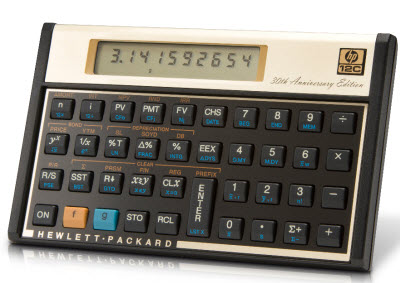
\includegraphics[width=90mm]{hp-calc-4.jpg}
\caption{The 30th Anniversary Edition of the HP 12C}
\label{overflow}
\end{figure}

\pagebreak

\section{Introduction}
\label{Introduction}

The HP 12C calculator has withstood the test of time.  It was first introduced by Hewlett Packard in 1981, and is still considered the preferred calculator of use by many individuals in the business and financial world.   It is a part of the HP 10C series, which also included the HP 15C calculator for advanced scientific functions and the HP 16C calculator for computer programming functions.  Due to the HP 12C’s popularity, the calculator remains in production today, with minor hardware updates throughout the years.  It is considered Hewlett Packard’s best selling product, although HP has never released official sales numbers.  When compared to any other technological innovation of its time, very few, if any at all, are still as popular as the HP 12C.  The following paper will explore the successful alignment of user and developer mental models of the HP 12C by analyzing the 5 usability metrics defined by Neilson in Usability Engineering.

\section{The Computational Environment of 1981}
\label{The Computational Environment of 1981}

The computer landscape of 1981 was drastically different compared to today’s landscape.  In order to understand the initial success of the HP 12C calculator, it is beneficial to analyze the early stages of the personal computer revolution.  The Altair 8800, the Apple II, and the Casio Mini Card LC-78 will be analyzed to acquire a sense of the computer environment of the 70’s and early 80’s, which will further the understanding of the HP 12C’s seemingly eternal success.\\

The Altair 8800, developed around the popular Intel 8080 processor of the time, was introduced in 1975.  It was one of the first computers marketed as a kit for hobbyists.  At the time it was first introduced, it had no programming language other than machine language.  A programmer would have to enter the machine language opcode manually by toggling a series of binary external switches, and use an enter switch to load the opcode into memory.  This process was extremely inefficient and impractical for any type of real world application.  Therefore, the Altair only appealed to self acclaimed computer hobbyists as a way to learn how to build a computer bit by bit (excuse the pun).\\

However, the Altair did boast an 8-bit Intel 8080 microprocessor, which had a clock speed of 2 MHz, making it one of the fasted processors of its time.  Because it was a hobbyist computer, it also had a low price point of 439.   These two factors opened up doors to outside visionaries like Bill Gates, who developed a version of BASIC for the Altair. This allowed a user to easily load programs into the Altair, like a mathematical operation.  This drastically improved user efficiency, and thus was the inception of Microsoft.\\

Another computer product of the time, the Apple II, which was launched in 1977, was Apple’s first mass-produced personal computer.  It contained a 1 MHz CPU and 4 KB of RAM.  Interestingly, the Apple II had a slower clock speed when compared to the Altair 8800, launched 2 years prior.  What made the Apple II popular was its color graphical display, its mouse driven GUI, and expansion slots for third party devices, among other things.  But the real driving factor for the Apple II’s success was the development of third party software, including VisiCalc, the first spreadsheet software that was launched in 1979.  Unlike the Altair, the Apple II was expensive, with an original retail price of 1298.  Yet, it was cheap enough to get it into a few homes and offices.\\

These two personal computers were revolutionary for their time, and it wasn’t until much later when personal computers became common in the home and workplace.  The world of hand held calculators developed in parallel with personal computers, yet experienced more success in the late 70’s and early 80’s with respect to popularity.  In general, pocket calculators were cheaper and more mobile than personal computers.  Manufacturers of pocket calculators in the 70’s and 80’s included HP, Canon, Texas Instruments, Mostek, Sinclair, Casio, Sanyo, and many others.  Therefore, the competition was steep, whereas the personal computer environment was still blossoming.\\

The first credit card sized calculator, the Casio Mini Card LC-78, was released in 1978, and measured a mere 3.9 mm thick.  It originally sold for 34.  This attractively thin form factor parallels today’s product design.  But the functionality of the Casio Mini Card was limited to basic arithmetic operations.  Users in the professional field needed calculators to compute specific functions to their fields of study.  This is where the HP 12C calculator comes into play.  The quantity of built in functions found in the HP 12C for financial applications made it a go to calculator for the business world.  But this does not explain how it has withstood the test of time, as those functions became a commonplace when spreadsheet software and future calculators flooded the marketplace.


\section{Functionality of the HP 12C}
\label{Functionality of the HP 12C}

What made the HP 12C so popular is its built in financial functionality.  These functions include common financial mathematical formulas like interest rate functions, bond functions, depreciation functions, statistical functions (mean, standard deviation, linear estimation etc.), real estate functions, and other miscellaneous financial related functions.  As a financial calculator, the user expects a set of functions.\\

With so much functionality, there is the risk of the user experiencing information overload, and becoming lost in the options of button pressing.  There are a total of 39 buttons on the HP 12C.  Submenus are created by the use of the f and g buttons.  This hides less used functionality of the calculator, or more advanced functionality of the calculator, depending on how one looks at it.\\

The industrial design of the product surpassed any other calculator of its time.  The calculator is durable and has a formal aesthetic quality, which blends in well on any CEO’s desk.  The colors of the calculator are warm and golden, which adds to the formality of the calculator.  The buttons stick out a substantial amount and are beveled at the bottom, giving it a more pyramidal shape.  This gives the calculator a good tactile response, which gives the user instant gratification.  There is never any doubt if the button was pressed or not pressed.\\

There is more to the calculator than its high level of functionality.  It uses Reverse Polish Notation (RPN), as opposed to the more commonly used algebraic notation.  RPN allows the user to input less keystrokes than algebraic notation.  RPN works by the user inputting the operands, which are followed by the operator.  For example to calculate 3 + 4, the following would be inputted into the calculator,\\

\centerline{[ 3 ] [ enter ] [ 4 ] [ + ]}
\

Contrast that with algebraic notation,\\

\centerline{[ 3 ] [ + ] [ 4 ] [ enter ]\linebreak}
\

At first it may be unclear how RPN would reduce the number of keystrokes as this example shows both notations use 4 keystrokes.  Therefore, let us look at an algebraic equation that requires knowledge of precedence (remember PEMDOS: Parentheses Exponentiation Multiplication Division Addition Subtraction).




\section{Industrial Design of the HP 12C}
\label{Industrial Design of the HP 12C}

\section{Reverse Polish Notation}
\label{Reverse Polish Notation}

\section{Conclusion}
\label{Conclusion}

\end{document}